\documentclass{article}
\usepackage{amsthm}
\usepackage{algpseudocode} 
\usepackage{graphicx}
\usepackage{hyperref}

\theoremstyle{definition}
\newtheorem{definition}{Definition}

\theoremstyle{definition}
\newtheorem{algorithm}{Algorithm}

\theoremstyle{theorem}
\newtheorem{claim}{Claim}
\newtheorem*{lemma}{Lemma}

\title{Minesweeper Solver Analysis}
\author{Jacob Slagle}

\emergencystretch 3em%
\begin{document}
	\date{}
	\maketitle
	
	\tableofcontents
	
	\section{Introduction}
	This document discusses in detail my thought process in developing the algorithms to solve a game of minesweeper, and serves as a write-up for a larger project - see my \href{https://github.com/slaglj/minesweeper_solver}{github repository}.\footnote{\url{github.com/slaglj/minesweeper_solver}} Along the way I derive asymptotic bounds and  prove the correctness of the algorithms, as well as completeness where applicable. 
	
	\subsection{Motivation}
	I did this project as an exercise and also for the heck of it. I chose Minesweeper because it would be a simple enough problem to keep the scope of the project in check, but on the other hand, not so simple that the algorithms would be completely trivial. 
	\section{Human-like Solving}
	Henceforth I will mostly stick to the formal "we" as in mathematical writing.
	
	To begin with we consider the problem of beating a game of minesweeper. Simply put, we are trying to decide which squares have mines and which do not. If we can find some such squares we flag the ones that have mines and reveal or "click" the squares that don't. In doing so, we gain information which helps us find more squares in turn. Assuming we can keep finding squares, eventually we'll cover the whole board and win the game
	
	For inspiration, we consider how a person plays minesweeper (as opposed to a computer executing an algorithm). If I can formalize the strategies I use to play minesweeper, I can turn them into an algorithm. \footnote{"I" instead of "we" here since I don't assume everyone plays minesweeper the way I do.}
	
	\subsection{The Strategies}
	When I play minesweeper, my bread and butter strategy is to consider the information provided a by looking at a number on the board, or by looking at two numbers in conjunction and seeing if I can deduce where mines must be, or where mines must not be. Consider this example:
	\begin{center}
		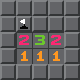
\includegraphics[width=0.2\textwidth]{exampleimages/example1a}
	\end{center}
	 There is a 3 on the board with only one flag next to it and exactly two blank squares next to it (i.e. the other five squares adjacent to it have been revealed).The 3 requires two more flags to satisfy it, and since only two blank squares adjacent to 3 remain we know those must contain mines and so we flag them
	\begin{center}
		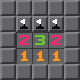
\includegraphics[width=0.2\textwidth]{exampleimages/example1b}
	\end{center}
	In doing so we are following a certain strategy: if the number of spaces around a number equals the number of flags that still need to be placed around it, then flag all those spaces. We now formalize that strategy. Let $p$ be a point on the board, and let $m$ be the number of mines around $p$ that need to be flagged beyond those that have already been flagged, and let $B$ be the blank squares adjacent to $p$ (in the above example, $m = 2$ and $|B| = 2$). We state the strategy in a pseudocode snippet:
	\begin{algorithmic}
		\If{$m = |B|$} \Comment strategy 1
		\State flagAll($B$)
		\EndIf
	\end{algorithmic}
	We also know that if there are no more flags required, then we can simply reveal all adjacent squares
	\begin{algorithmic}
		\If{$m = 0$} \Comment strategy 2
		\State revealAll($B$)
		\EndIf
	\end{algorithmic}
	
	Those are the two strategies we follow when we look at one number. Now consider this example, where we need to look at two numbers:
	\begin{center}
		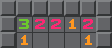
\includegraphics[width=0.3\textwidth]{exampleimages/example2a}
	\end{center}
	Consider the 2 in the center and the 1 directly to the right of it. There are two squares adjacent to both of them, the space above the 2 and above the 1. Because these squares are adjacent to the 1, only one of them can contain a mine. But the 2 must have two mines adjacent to it, and so there must be another mine elsewhere to satisfy it. Outside of these two spaces shared by the  1 and the 2, the only blank square is above and to the left of the 2, so we flag this space:
	\begin{center}
		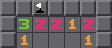
\includegraphics[width=0.3\textwidth]{exampleimages/example2b}
	\end{center}
	To capture this idea in a strategy we define some variables: Iet $p_1$ and $p_2$ be two points on the board, let $m_1$ and $m_2$ the number of mines needed to satisfy $p_1$ and $p_2$ respectively, and let $B_1$ and $B_2$ be the blank squares around $p_1$ and $p_2$ respectively. Set $I = B_1 \cap B_2$.  Observe that since $I \subseteq B_1$ it can not contain any more mines than $B_1$ which contains $m_1$ mines, that is $I$ can not contain more than $m_1$ mines. We can apply the same logic with $B_2$ instead of $B_1$ to say  $I$ contains no more than $m_2$ mines. $I$ of course can not contain more than $|I|$ squares, and combining all this we can define an upper bound $i_{max}$ on the number of mines in $I$
	$$i _{max} = \textrm{max}(m_1,m_2,|I|) $$
	With these definitions we state another strategy
	\begin{algorithmic}
		\If{$m_1 - i_{max} = |B_1 - I|$} \Comment Strategy 3
		\State flagAll($B_1 - I$)
		\EndIf
	\end{algorithmic}
	as well as the symmetric strategy
	\begin{algorithmic}
		\If{$m_2 - i_{max} = |B_2 - I|$} \Comment Strategy 4
		\State flagAll($B_2 - I$)
		\EndIf
	\end{algorithmic}
	If we call the 1 in our example $p_1$ and the 2 is $p_2$, then the strategy we used in the example above is Strategy 4. 
	
	We can also establish a \textit{lower} bound, $i_{min}$, on the number of flags in $I$. Namely, $B_1 - I$ can only contain $|B_1 - I|$ mines, and so $I$ must contain the remaining $m_1 - |B_1 - I|$ mines required around $p_1$. Similarly $I$ must contain at least $m_2 - |B_2 - I|$ mines, and so we say
	$$i_{min} = \textrm{max}(m_1 - |B_1 - I|, m_2 - |B_2 - I|)$$
	Using this we derive three more strategies:
	\begin{algorithmic}
		\If{$i_{min} = |I|$} \Comment Strategy 5
		\State flagAll($I$)
		\EndIf
	\end{algorithmic}
	\begin{algorithmic}
		\If{$i_{min} = m_1$} \Comment Strategy 6
		\State revealAll($B_1 - I$)
		\EndIf
	\end{algorithmic}
	\begin{algorithmic}
		\If{$i_{min} = m_2$} \Comment Strategy 7
		\State revealAll($B_2 - I$)
		\EndIf
	\end{algorithmic}
	In fact, if we apply Strategy 6 to our example (with $p_1$ as the 1 and $p_2$ as the 2, as before), we are able to reveal a square:
	\begin{center}
		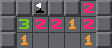
\includegraphics[width=0.3\textwidth]{exampleimages/example2c}
	\end{center}
	
	\subsection{Human-like Algorithm }
	The basic idea for the algorithm is to just apply to the strategies to different points (or pairs of points) on the board until the game is won. It's just a matter of deciding when and where to apply the strategies. Note that when two points $p_1$ and $p_2$ do not have any blank neighbors in common there is no point in applying strategies 3-7: in this case $I = \emptyset$ so Strategy 5 does nothing, Strategies 3 and 6 reduce to Strategies 1 and 2 with $p = p_1$, and Strategies 4 and 7 reduce to Strategies 1 and 2 with $p = p_2$. With this in mind, we write a subroutine that takes a point $p$ and applies all the necessary strategies to it.
	\newpage
	\begin{algorithmic}
		\Function{ApplyStrategies}{$p$}
		\State Apply Strategies 1 and 2 to $p$
		\State $p_1 \gets p$
		\ForAll{points $p_2$ that share a blank neighbor with $p_1$}
		\State Apply Strategies 3-7 to $p_1$ and $p_2$
		\EndFor
		\EndFunction
	\end{algorithmic}
	Now its just a question of which points to call ApplyStrategies on. Firstoff, we only need to check revealed points, i.e. squares with numbers. Secondly we only need to bother with points that have at least one blank neighbor- we will call the collection of all such points the \textbf{fringe} because it consists of those squares on the edge of the contiguous blob(s) of revealed squares. Finally, while we may need to call ApplyStrategies repeatedly on a given point $p$, we only need to call it again \textit{after} one of the blank neighbors of $p$ has been flagged or revealed. To capture this we'll have a variable active (we use a stack, but any collection suffices) which tracks which points need to be checked. Here is the pseudocode to solve a game $G$ of minesweeper. We assume at least one move has been made so that there are revealed squares and a fringe to begin with \footnote{With a new game there is essentially no strategy in choosing the first move. The intent of the algorithm is solve a game after a (random) first move is made, or for that matter, any game in progress. Most implementations of Minesweeper guarantee that the first move is not fatal, and some even guarantee that a whole blob is revealed to give the player a fighting chance- this includes the implementation in my project.}
		\begin{algorithmic}
		\Function{HumanSolve}{$G$} \Comment Human-Like algorithm
		\State $active \gets$ fringe of $G$
		\While{$active$ is not empty}
		\State $p \gets active.\textrm{pop()}$
		\State ApplyStrategies($p$)
		\ForAll{revealed points $q$ with a just revealed/flagged neighbor}
		\State $active$.push($q$)
		\EndFor
		\EndWhile
		\EndFunction
	\end{algorithmic}

	
	\subsubsection{Correctness and Completeness}
	The algorithm is correct in the sense that when it identifies a mine or a free square it does so correctly, and so can "correctly" win a game. A formal proof of this would just be a reiteration of the above discussion. However there is no guarantee that it will beat the game, and as we discuss below there are games that are theoretically solvable which are not solved by this algorithm.
	\subsubsection{Space and Runtime}
	The only significant space usage is in the variable $active$ which is of course bounded by the number of points $b$ on the game board, so the algorithm uses $O(b)$ space.
	
	Observe that each strategy can be applied in constant time. Moreover all the points $p_2$ must be within two squares of $p_2$, and there are 25 such squares (within a five by five window centered around $p_1$). It follows that ApplyStrategies executes in constant time. Fix a point $p$. ApplyStrategies might be called on $p$ once and then each time a point adjacent to it is revealed. There are only 8 points adjacent to $p$, so in total ApplyStrategies can be called up to 9 times on $p$. Thus this algorithm runs in $O(b)$ time, where again $b$ is the number of points on the game board.
	
	\section{What about completeness?}\label{whatabout}
	The algorithm outlined above works pretty well and is pretty efficient, however as we mentioned above it is not complete . Consider this example of a game in progress:
	\begin{center}
		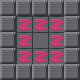
\includegraphics[width=0.2\textwidth]{exampleimages/example3a}
	\end{center}
	If we run the human-like algorithm here we make no progress- no flags and no reveals. As it turns out there is a unique solution here:
	\begin{center}
		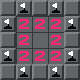
\includegraphics[width=0.2\textwidth]{exampleimages/example3b}
	\end{center}
	Perhaps our algorithm would be able to make more progress if we added another strategy, maybe one that takes into account more than two squares at a time? Indeed by looking at, say the, the 2 in the top right corner as well as the 2 it's left and the 2 to directly below it we could conclude that the top right corner contains no mine (the 2 in the corner must share at least one mine with each of the other 2's. This accounts for both of the mines that the corner 2 requires, but neither of these mines can occupy the top right corner of the board, and so it must be free). By symmetry all the corners must be blank. So we were able to reveal four more squares in this way. In fact by looking at five squares at a time we can determing which of the remaining squares are also free and thus win the game (we spare the details).
	
	As it stands the human-like algorithm is incomplete in the sense that one could solve the above example game, but this algorithm fails to. Is there a way to add strategies to \textit{make} the algorithm complete tho? For instance adding two more strategies would allow the algorithm to solve the above game. 
	
	The fact is that trying to combine the imformation from five or even just three numbers is not straightforward or clean. Working out all of the different possible strategies becomes a lot more complicated when looking at more than two points, and so adding Strategies isn't the trick. Rather than looking at particular subsets of numbers, it might be worth it to just look at all the numbers at once. In the next section we develop an algorithm that does just that.
	\section{Exhaustive Solving}
	As a starting point we consider what exactly it means to beat a game of minesweeper. To win we must place flags on exactly those squares which contain mines and reveal the rest of the squares- in other words we must find the right "placement" of flags on the board. We say a  \textbf{frame} of a game is a freeze frame of a game in progress, i.e. a frame is an array of squares representing the game board where each square is marked as flagged or blank, or is revealed and displying a number (0's are implicit and are shown simply as depressed squares). Because those numbers tell us how many mines there are adjacent to it, we call them \textbf{hints}. A \textbf{placement} is a subset of the blank squares on the board which we regard as a possible way of placing additional flags to designate where mines are. Since we aim to place flags on mines and only mines, these hints are constraints on the way flags can be placed. With an eye towards satisfying these constraints, we make the following definition:
	\begin{definition}
		A placement is \textbf{satisfactory} if after placing all flags in it we have this property: for every revealed square $s$, the number hint $h$ in $s$ is equal to the number of flags surrounding $s$.
	\end{definition}
	Observe that the correct placement of flags on mines is itself a satisfactory placement, which we call the \textbf{actual placement}. It follows that if a square is flagged in \textit{every} satisfactory placement, it must contain a mine, because in particular it is flagged in the actual placement. Therefore we say placing a flag on such a square is a \textbf{certain flag} (a flag placed with certainty). Likewise, if a square is \textit{unflagged} in every mine placement, we know it must be free (i.e. it does not contain a mine). Thus we say revealing it is a \textbf{certain reveal}. A \textbf{certain move} is a certain flag or a certain reveal. 
	
	Consider the value of a certian move over an uncertain move: in playing Minesweeper, we do not know where the mines are but we \textit{can} figure out what the satisfactory placements are by looking at hints, and so can deduce certain moves. Moreover we really \textit{have} to resort to looking only at certain moves because if a reveal is uncertain, there are satisfactory placements in which the revealed square contains a mine, and if one of those satisfactory placements is the actual placement then revealing the square loses the game. Uncertain flags, while not immediately fatal, can lead to errors down the line. Hence we only want to make certain moves. This line of reasoning lends itself to an algorithm.
	\subsection{Brute Force Algorithm}
	Note that this algorithm does not try to solve the game in its entirety, but rather tries to solve a "frame" of the game. To solve the game, we need to apply this version of solve repeatedly.
	
	 Simply put, we need to generate all satisfactory placements, check which squares are consistently flagged (and are thus certain flags) or unflagged (certain reveals) across each placement and make certain moves accordingly. Let's assume for the moment we have a function satisfactoryPlacements($G$) which takes a game of minesweeper $G$ and generates all satisfactory placements. Here is the algorithm in pseudocode:
	\begin{algorithmic}
		\Function{BruteSolve}{$G$}  \Comment Brute force algorithm
		\State $Mines \gets$ game board
		\State $Free \gets$ game board
		\For{$P$ in satisfactoryPlacements($G$)}
		\State $Mines \gets Mines \cap P$
		\State $Free \gets Free -  P$
		\EndFor
		\State flagAll($Mines$)
		\State revealAll($Free$)
		\EndFunction
	\end{algorithmic}
	We just need to implement satisfactoryPlacements(). We start with a brute force approach: go over all mine placements and yield the ones that are satisfactory. Mine placements are just subsets of the game board $B$, i.e. elements of the powerset $\mathcal{P}(B)$.
	
	\begin{algorithmic}
		\Function{satisfactoryPlacements}{$G$}
		\For{$P$ in $\mathcal{P}(B)$}
		\If{$P$ is satisfactory}
		\State \textbf{yield} $P$
		\EndIf
		\EndFor
		\EndFunction
	\end{algorithmic}
	
	We leave 
	
	\subsubsection{Correctness and Completeness}
	Regarding correctness, we reiterate our discussion above.The algorithm only flags squares in the intersection of all satisfactory placements, which is a subset of the actual placement. It only reveals squares that are not a part of any satisfactory placement, in particular they are not a part of the actual placement.
	
	In the discussion of our human-like algorithm we alluded to the fact that in a certain sense it was not complete, and we can now state more precisely what we meant. Our notion of completeness is nuanced, because it does not mean the algorithm always beats the game. In general completeness means that when there is a solution the algorithm finds it. For our purposes we will say there is a solution when there is at least one certain move to be made. (This definition puts solution in terms of frames, not in terms of the game as a whole). We gave an example above where there are certain moves to be made (where in fact the game could be beaten) which the human-like algorithm did not find. In this sense the human-like algorithm is incomplete. On the other hand our brute algorithm was created explicitly to find all certain moves, and so is complete.
	
	\subsubsection{Space and Runtime}
	 This method checks $|\mathcal{P}(B)| = 2^{b}$ placements, where $b = |B|$ is the size of the board. We can check if a placement is satisfactory in linear time, and since the placements are bound by the board size, we have that satisfactoryPlacements() has an $O(b2^{b})$ runtime. The other work in solve is relatively insignificant and so this also the runtime for solve(). We must apply solve() repeated to actually beat the game. We can't assume that solve() makes move on more than one square for each call, so the beat the game takes up to $b$ applications of solve(), or $O(b^22^{b})$.
	 
	 As far as space, if we regard SatisfactoryPlacements() as a generator a la Python (which is in fact how it is implemented in my code), then all variables are bounded in size by the game board, and so the algorithm uses $O(b)$ space.
	 
	 \subsection{Idea: Reducing Scope}
	 An $O(b^22^{b})$ runtime is pretty bad, but there's a reason we call this the brute force algorithm. Here we consider one way to make it more efficient.
	 
	 If you've ever played minesweeper though it might occur to you that it's unecessary to look at the entire board, since in a sense we only have information about the blank squares which are adjacent to revealed squares (hints). With this in mind we make the following definitions: a square is \textbf{in-play} if (in the frame in question) it is unrevealed and unflagged and adjacent to a revealed square. We will refer to all in-play squares collectively as the \textbf{perimiter} because they circumscribe the revealed part of the board (different from the fringe, defined above). We will make the algorithm more efficient by reducing the scope of the algorithm to the perimiter.
	
	\begin{lemma}
		If $S$ is a satisfactory placement and $P$ is the perimiter,  then $S' = S \cap P$ is also a satisfactory placement.
	\end{lemma}

	\begin{proof}
		Let $r$ be a revealed square. All the flags in $S$ adjacent to $r$ are also in $S' = P \cap S$ because the perimiter $P$ contains all the in-play squares in the current frame. In particular $r$ has the same number of flags adjacent to it in $P'$ as in $P$. This goes for each revealed square $r$, so $S'$ like $S$ is a satisfactory placement.
	\end{proof}
	\begin{claim}
		
		
		\begin{enumerate}
		
		\item
		A flag is certain if and only if it occurs in each satisfactory placement contained within the perimiter. Additionally, certain flags always occur within the perimiter
		
		\item
		A reveal is certain if and only if it is in the perimiter and the space to be revealed is unflagged in each satisfactory placement contained within the perimiter.
		
		\item
		Certain moves occur only in the perimiter of the board.
		\end{enumerate}
	\end{claim}

	\begin{proof}
	\begin{enumerate}
		\item
		If a flag is certain if it is contained in every satisfactory placement, in particular it is a part of the satisfactory placements contained within the perimiter. Conversely, suppose $s$ is a space that is flagged in every satisfactory placement that is contained within the perimiter. Let $S$ be an arbitrary satisfactory placement. Set $S'$ be the intersection of $S$ and the perimiter. By the lemma, $S'$ is also satisfactory, and so by our hypothesis,  $s \in S'$. Of course $S' \subset S$, and so $s \in S$. Thus $s$ is in every satisfactory placement $S$, meaning $s$ is a certain flag. This proves the iff statement. 
		
		To prove that all certain flags are in the perimiter let $M$ be the actual mine placement, which is satisfactory (for the purposes of this proof $M$ could be any satisfactory mine placement). By the lemma $M' = M \cap perimiter$, the intersection of $M$ and the perimiter, is satisfactory. By the definition of certain, all certain flags are in $M'$ which is  in the perimiter.
		
		\item
		Suppose $s$ is a certain reveal. By definition then, $s$ is not contained in any satisfactory mine placement, in particular those contained within the perimiter. Suppose for contradiction $s$ was not in the perimiter. Let $M$ be the actual mine placement (or any satisfactory mine placement for that matter), and set $M' = M \cup \{s\}$. Since $s$ is not in the perimiter it is not in play meaning that adding it to a placement would not change the number of flags around any revealed square. In particular adding it to $M$ would yield a placement $M' = M \cup \{s\}$ which had the same flag counts around each revealed square, i.e. another satisfactory placement. Thus $s$ is in a satisfactory placement $M'$, which is a contradiction because $s$ is a certain reveal.
		
		Conversely, suppose $s$ is in the perimiter and is unflagged in each satisfactory placemnt contained within the perimiter. Let $S$ be a satisfactory placement, and let $S'$ be it's intersection with the perimiter. By the lemma, $S'$ is a satisfactory placement, and so by out hypothesis $s \notin S'$. But since  $s$ is in the perimiter and $S'$ is the intersection of $S$ with the perimiter, the only way $s \notin S'$ is if $s \notin S$. This shows that $s$ is contained in no satisfactory placement and so by definition $s$ is a certain reveal.
		
		\item
		This statement follows immediately from the first two.
		
		
	\end{enumerate}
	\end{proof}

	This claim shows us that our algorithm need only focus on the perimiter as opposed to the whole board. That is, we can initialize the variables $Mines$ and $Free$ to be just the perimiter and we only need to generate satisfactory placements that are contained within the perimiter. Here are the revised versions of BruteSolve() and satisfactoryPlacements():
	
	\begin{algorithmic}
		\Function{BruteSolve}{$G$} \Comment Version 2
		\State $Mines \gets$ perimiter of $G$
		\State $Free \gets$ perimiter of $G$
		\For{$P$ in satisfactoryPlacements($G$)}
		\State $Mines \gets Mines \cap P$
		\State $Free \gets Free -  P$
		\EndFor
		\State flagAll($Mines$)
		\State revealAll($Free$)
		\EndFunction
	\end{algorithmic}
	
	\begin{algorithmic}
		\Function{SatisfactoryPlacements}{$G$} \Comment Version 2
		\For{$P$ in $\mathcal{P}$(perimiter of $G$)}
		\If{$P$ is satisfactory}
		\State \textbf{yield} $P$
		\EndIf
		\EndFor
		\EndFunction
	\end{algorithmic}

	\subsubsection{Correctness and Completeness}
	The claims above establish that correctness and completness are preserved after we reduce the scope of the algorithm.
	
	\subsubsection{Space and Runtime}
	This reduces the runtime of BruteSolve() to $O(p2^{p})$ where $p$ is the size of the perimiter. While this is still exponential, the perimiter tends to be much smaller than the board. To wave my hands for a moment: the board has 2 dimensions while the perimiter is more like a 1-dimensional curve embedded in it. In the worst case we still need to apply solve $b$ times, so we would say that it takes $O(bp2^p)$ time to beat the game except that this is an abuse of notation: $p$ is a constant for each \textit{frame} of the game, but the perimter changes as more moves are made. Techinically we can still only say that the runtime to solve a whole game (not just one frame) is $O(b^22^b)$.
	
	Space used per frame is $O(p)$, and over the course of the game is $O(b)$.
	
	\subsection{Idea: Building Satisfactory Placements}
	Even when we restrict our attention to the perimiter, it seems like we're doing exta work when we go back and check if a placement is satisfactory- after all this is where the linear factor $p$ in $O(p2^{p})$ comes from. What if rather than looking at every placement, we "built up" satisfactory placements according to the hints on the board. If we build placements correctly, we don't have to check that they are satisfactory. Recall this term: the \textbf{fringe} consists of all revealed squares (numbers) with at least one adjacent blank square. Note the distinction between the fringe and the perimiter: the fringe consists of the edge (or edges), of the revealed part(s) of the board, while the perimiter is unrevealed and wraps around the fringe. Functionally speaking the fringe contains all the hints on the board that have yet to be satisfied, and as such is our focus if we are building up satisfactory placements.
	
	To give a rough idea of the algorithm, the core idea is to look at a point in the fringe and add the appopriate number of flags around it to satisfy it. There are usually multiple ways to add the appropriate number of flags, so we choose one  way and proceed to the next point, doing the same with this point. We continue in this manner until we have a satisfactory placement, which we then yield. We then backtrack an consider other ways of adding flags around points.
	
	\subsection{Recursive Backtracking Algorithm}
	For this change we are only updating the SatisfactoryPlacements function, which we can simply plug into Version 2 of the BruteSolve() function. As the title of this section implies, it is a recursive backtracking algorithm.
	
	\begin{algorithmic}
		\Function{SatisfactoryPlacements}{$G$} \Comment Version 3
		\State SPHelper($G,0, \emptyset$)
		\EndFunction
		
		\Function{SPHelper}{$G,i,placement$}
		\If{$i =$ length($G.fringe$) } \Comment recursion base case
		\State \textbf{yield} $placement$
		\EndIf
		\State $point \gets G.fringe[i]$ \Comment Get the $i$th point in the fringe
		\If{$point$ has too many flags around it when including those in $placement$}
		\State return \Comment Go back up one level of the call stack
		\ElsIf{$point$ already has the right number of flags around it}
		\State SPHelper($G, i+1, placement$)
		\Else
		\ForAll{sets of flags $newFlags$ that can be added to satisfy $point$ without adding flags around $G.fringe[0], G.fringe[1]$,...,$G.fringe[i-1]$}
		\State $placement \gets placement \cup newFlags$
		\State SPHelper($G, i+1, placement$)
		\State $placement \gets placement - newFlags$
		\EndFor
		\EndIf
		
		\EndFunction
	\end{algorithmic}

	\subsubsection{Correctness and Completeness}
	As we have shown already, to prove the correctness and completeness of the algorithm it suffices to show that SatisfactoryPlacements() generates all satisfactory placements within the perimiter.
	\begin{claim}
		The above version of SatisfactoryPlacements() yields exactly those satisfactory placements contained within the perimiter.
	\end{claim}
	\begin{proof}
		The perimiter is just the union of all in-play squares adjacent to points in the fringe, so we might rephrase the claim as SatisfactoryPlacements() yields exactly those satisfactory placements that contain only flags adjacent to points in the fringe. Now consider the following propositions which depends on the variable $k$.
		
		\bigskip
		OnlySatisfactory($k$): Whenever a call of the form SPHelper($G,k,placement$) is made, which is to say a call with $i = k$, then the variable $placement$ is a placement that satisfies \footnote{A placement \textbf{satisfies} a point if after placing flags from said placement, said point has exactly the required number of flags around it. Per our definition of satisfactory placement above, a satisfactory placement is one that satisfies all points in the fringe} the points $G.fringe[0],...,G.fringe[k-1]$
	
		\bigskip
		 AllSatisfactory($k$): Each placement which (a) satisfies the points $G.fringe[0]$, ...,$G.fringe[k-1]$ and (b) contains only flags adjacent to $G.fringe[0], ..., G.fringe[k-1]$ is stored in the variable $placement$ at the beginning of one of the function calls of the form SPHelper($G,k,placement$)
		 
		 \bigskip
		 The statement OnlySatisfactory(length($G.fringe$)) should be interpreted as follows: when the base case of the recursion is entered (because $i$ equals length($G.fringe$)) the $placement$ variable contains a satisfactory placement because all points in $G.fringe$ are satisfied, and thus the placement that's yielded is satisfactory. The statement AllSatisfactory(length($G.fringe$)) guarantees  that all satisfactory placements contained within the perimiter are yielded. Together these statements tell us that SatisfactoryPlacements() yields exactly those satisfactory placements contained within the perimiter, which is our goal. We prove OnlySatisfactory(length($G.fringe$)) and AllSatisfactory(length($G.fringe$)) by induction on $k$.
		 
		There are no points to be satisfied in base case ($k = 0$), so OnlySatisfactory(0) is trivial. Recursive calls are made with strictly ascending values of $i$, so SPHelper() is only called once with $i = 0$ once and in this  case $placement = \emptyset$. Indeed $\emptyset$ is the only placement which fulfills conditions (a) and (b) in AllSatisfactory(0)
		
		Now suppose OnlySatisfactory($k$) is true. Calls of the form SPHelper($G,k+1,placement$) are only made within calls of the form SPHelper($G,k,placement$). When such a call is made from the else if clause, then $placement$ already satisfies the hint at point $G.fringe[k]$ and OnlySatisfactory($k$) tells us that it also satisfies $G.fringe[0], ..., G.fringe[k-1]$. This establishes the statment OnlySatisfactory($k+1$) for the if else clause. Otherwise the call SPHelper($G,k+1,placement$) is made within the for each loop. Adding $newFlags$ to $placement$ guarantees that $placement$ satisfies $G.fringe[k]$, but by the condition in the for each loop $newFlags$ doesn't contain any flags around $G.fringe[0], ..., G.fringe[k-1]$. OnlySatisfactory($k$) guarantees that $placement$ satisfied $G.fringe[0], ..., G.fringe[k-1]$ to begin with, and after adding $newFlags$ which doesn't contain any flags around these points, they continue to be satisfied. Thus OnlySatisfactory($k + 1$) is true.
		
		Now suppose AllSatisfactory($k$) is true. Let $P$ be a placement as described in AllSatisfactory($k+1$).  Let $N$ be the flags from $P$ which are adjacent to $G.fringe[k]$ but are not adjacent to $G.fringe[0], ..., G.fringe[k-1]$($N$ may be empty), and set $P'$ equal to $P - N$. $P'$ is one of the placements described in AllSatisfactory($k$), and so there is a call of the form SPHelper($G,k,placement$)  with $placement$ equal to $P'$. If $N = \emptyset$ then $placement = P' = P$ satisfies $G.fringe[0], ..., G.fringe[k]$ already and the else if clause makes the call SPHelper($G,k + 1,placement$) as required. Otherwise if $N \neq \emptyset$, one of the iterations of the for each loop sets $newMines$ equal to $N$ and adds $newMines$ to $placement$. Since $placement$ equals $P'$ before this it now equals $P' \cup N = P$. Thus SPHelper($G,k + 1,placement$) is called with $placement = P$ as desired.
	\end{proof}

	\subsubsection{Space and Runtime}
	Let $p$ be the size of the permiter and $f$ the size of the fringe.
	\begin{claim}
		$O(p) = O(f)$
	\end{claim}
	\begin{proof}
	By the definitions of fringe and perimiter, the permite consists of exactly the points adjacent to points in the fringe. A point (in the fringe) only has 8 neighbors, so ther are only as many as $8f$ points in the perimiter, which is to say $p \leq 8f$. A symmetric argument shows that $f \leq 8p$ and the conclusion follows.
	\end{proof}
	
	Regarding space: the only significant variable in terms of space is $placement$, which is contained in the permiter, and so is $O(p)$ in size. SPHelper proceeds depth first and so the call stack is only ever as deep as the index $i$, Thus there are a maximum of $f$  calls on the call stack where $f$ is the size of the fringe, i.e. length($G.fringe$). Each call only stores an $O(1)$ reference to the variable $placement$ the call stack uses $O(f) = O(p)$ space. Thus overall space usage is $O(p)$
	
	Now onto runtime. First observe that each iteration of the for each loop in SPHelper() includes a recursive call, so we can associate the work done in this iteration as a a prt of the recursive call (i.e. we associate the work in the for loop with the call SPHelper($G, i+1, placement$, not with the current SPHelper($G, i, placement$ call). All other work done in a call to SPHelper is constant, thus the runtime is proportional to the number of calls to SPHelper. Now observe that the beginning of each call to SPHelper $placement$ stores a different subset of the perimiter (we will not bother to, but we could prove this by induction), and so the number of calls is bounded by the number of subsets of the perimiter, i.e. $2^p$ where $p$ is the size of the perimiter. Thus the runtime is $O(2^p)$.
	
	As desired we've dropped the factor of $p$ from the previous version of SatisfactoryPlacements(). Beyond a better asymptotic runtime though, there's an additional efficiency to this version that's not clear from asymptotic bound $O(2^p)$.  We can think of SatisfactoryPlacements as "searching" a tree where each node is a subset of the perimiter, that subset being stored in $placement$ as the algorithm proceeds. Each node at level $i$ of the tree is a subset that satisfies points $G.fringe[0],...,G.fringe[i-1]$. Adding flags to a node at level $i$ to satisfy $G.fringe[i]$ yields a child node at level $i + 1$. If we were not careful we would search the entire tree, which consists of $2^p$ nodes/subsets. However the algorithm specifically cuts off at the points where its unable to satisfy the next point $G.fringe[i]$ (the else if statement) and also never satisfies $G.fringe[i]$ in a way that would put too many flags around $G.fringe[0],...,G.fringe[i-1]$ (the condition in the for all statement). In this way the algorithm "prunes" the tree as it searches, so in some cases the algorithm runs much faster that $O(2^p)$. This is in contrast to our original implementation of SatisfactoryPlacements() which \textit{always} considered all $2^p$ subsets of the perimiter, on top of checking if it was satisfactory.
	
	
	
	
	
\end{document}